\documentclass[english,letter,12pt,onesided]{article}
\usepackage{amsfonts}
\usepackage[left=1in,right=1in, bottom = 1in, top=1in]{geometry}
\usepackage[utf8]{inputenc}
\usepackage{babel}
\usepackage{slantsc}
\usepackage{setspace} 
\usepackage{array}
\usepackage{amsmath}
\usepackage{amsthm}
\usepackage{amssymb}
\usepackage[pdftex]{color,graphicx}
\usepackage{enumerate}
%\usepackage{mathtools}
%\usepackage{natbib}
\usepackage{bbm}
\usepackage{tikz}
\usepackage{subfigure}
\usepackage{pgfplots}
\usepackage{utopia}
\usepackage[labelsep=period]{caption}
\usepackage{hyperref}
\usepackage{setspace}
\usepackage{url}

\usepackage{caption}
\usepackage{wrapfig}
\usepackage{eufrak}

\usepackage{graphicx}

\DeclareMathOperator*{\argmin}{arg\,min}

\setcounter{MaxMatrixCols}{10}

\usetikzlibrary{patterns,snakes}
\newtheorem{theorem}{Theorem}
\newtheorem{proposition}{Proposition}
\newtheorem{corollary}{Corollary}
\newtheorem{lemma}{Lemma}
\newtheorem{claim}{Claim}
\newtheorem{propapp}{Proposition}[section]
\newtheorem{corapp}{Corollary}[section]
\newtheorem{lemmaapp}{Lemma}[section]
\theoremstyle{definition}
\newtheorem{definition}{Definition}
\newtheorem{example}{Example}
\newtheorem{assumption}{Assumption}
\newtheorem{remark}{Remark}

\newcommand{\R}{{\mathbb{R}}}
\newcommand{\Q}{{\mathcal{Q}}}
\newcommand{\Z}{{\mathbb Z}}
\newcommand{\Ce}{{\mathbb C}}
\newcommand{\N}{{\mathbb{N}}}
\newcommand{\G}{{\mathcal{G}}}
\newcommand{\K}{{\mathcal{K}}}
\newcommand{\V}{{\mathcal{V}}}
\newcommand{\E}{{\mathcal{E}}}
\newcommand{\M}{{\mathcal{M}}}

\newcommand{\ie}{{i.e., }}
\newcommand{\eg}{{e.g. }}
\newcommand{\ea}{{\it et al. }}
\newcommand{\st}{{\mathrm{s.t.}}}
\newcommand{\h}{{\text{H}}}
\newcommand{\w}{{\text{w}}}
\newcommand{\n}{{\mathbf{n}}}
\newcommand{\HT}{\mathcal{H}_{2}}
\newcommand{\HB}{\mathbf{H}}
\newcommand{\Tr}{\mathbf{Tr}}
\newcommand{\adj}{A_{\G}}
\newcommand{\hs}{\hspace{0.05cm}}

\newcommand{\NN}{\boldsymbol{\mathcal N}}
\newcommand{\RR}{\mathcal{R}}


\newcommand{\rhoo}{\rho_\text{ss}}
\newcommand{\rhoot}{\tilde{\rho}_\text{ss}}
\newcommand{\LK}{L_{_F}}
\newcommand{\Wc}{\varpi}
\newcommand{\wc}{w}
\newcommand{\wdet}{\varpi}
\newcommand{\Sp}{\hspace{0.05cm}}
\newcommand{\B}{\mathbf}
\newcommand{\BB}{\boldsymbol}
\newcommand{\ER}{\Xi_{\mathcal G}}
\newcommand{\PP}{\mathbb{P}}


\newcommand{\keywords}[1]{\par\addvspace\baselineskip
\noindent\keywordname\enspace\ignorespaces#1}
\definecolor{PennBlue}{RGB}{001,031,091}
\definecolor{PennRed}{RGB}{153,0,0}
\definecolor{NewBlue}{RGB}{001,031,110}
\definecolor{NewRed}{RGB}{200,0,0}
\hypersetup{
pdfborder = {0 0 0},
    colorlinks,
    citecolor=PennRed,
    filecolor=PennRed,
    linkcolor=PennRed,
    urlcolor=PennRed
}
\setcounter{secnumdepth}{2}

\setcounter{page} {1}



\begin{document}
\singlespacing
\begin{center}
\Large \textbf{Lehigh's Flying Machines Coliseum}
\end{center}
 \normalsize
\begin{wrapfigure}{r}{0.35\textwidth}
\center
    \includegraphics[width=0.35\textwidth]{IMAG1065} 
    \caption*{The LFMC is located at 1515 North Mountain Drive, BETHLEHEM, PA, 18015.}
\end{wrapfigure}

\noindent The theoretical outcomes of the proposed project will be implemented in Lehigh's Flying Machines Coliseum (LFMC) as part of Distributed Control and Dynamical Systems (DCDS) Laboratory, in the Department of Mechanical Engineering and Mechanics at Lehigh University. 

The mission of LFMC is to investigate experimental aspects of  advanced control capabilities for single or multiple/interconnected quad-copters. The DCDS Lab team is developing design methodologies to optimize drone size, flight controller, and on-board sensors by integrating and co-designing control and navigation algorithms. The group's vision is to unveil the fundamental principles of long-term autonomy.

\vspace{0.1in}
\noindent The LFMC was founded in 2017 as a part of the DCDS group and. Its mission regards experimental research on autonomous flying quad-copters. The overall facility measures up to 4000 square feet and it includes a platform for flying quadcopters, a conference/lab room, an auxiliary office as well as a facility station with a 24/7 running server.
\subsection*{The Platform} The main platform covers a space of approximately 3500 square feet. It is equipped with 16 high-precision Opti-Track motion capture system and 4 HD cameras. \begin{wrapfigure}{l}{0.35\textwidth} 
\center
    \includegraphics[width=0.35\textwidth]{IMAG1089} 
    \caption*{View of the surveillance system in the Platform room. It consists of the Opti-Track motion capture and the HD camera.}\vspace{-0.5in}
\end{wrapfigure} Real-time experiments are monitored via a high level operating station, that processes motion capture system data to control units using a wireless communication network. The platform space is supported by the server station and the conference/lab room. 



\subsection*{The Conference/Lab Room}
This is a classroom style room used for all non-aerial experimental activities. These activities regard construction and programming of drones, on either software or hardware layers. The space also serves as an observatory of the executed experiments that take place in the platform room, through a wide-screen TV that monitors the main area. The room is occasionally used for the DCDS group's teaching needs. It has so far hosted two graduate level courses of the Mechanical Engineering and Mechanics Department, relevant to the group's research interests.

\subsection*{The DCDS Armada}
The LFMC utilizes three types of drones, each on for different purposes. The small scale (mini) drones are used for basic calibrating/online testing of various embedded hardware, or for evaluating custom-made software algorithms. The second type is a custom-designed model, designed, constructed and assembled in our lab. It is geared for supporting the bulk of the group's current research activities. The last model is utilized for highly complex experimental tasks.   

\subsubsection*{The Crazepony} Crazepony is a really ultra-compact palm sized quadcopter kit for development, teaching and experimentation. This is an open source drone. Crazepony MINI Remote Controller is included, controlling the quadcopter through low-energy radio based on the nRF24L01+ chip.

\begin{figure}[t]
\center
    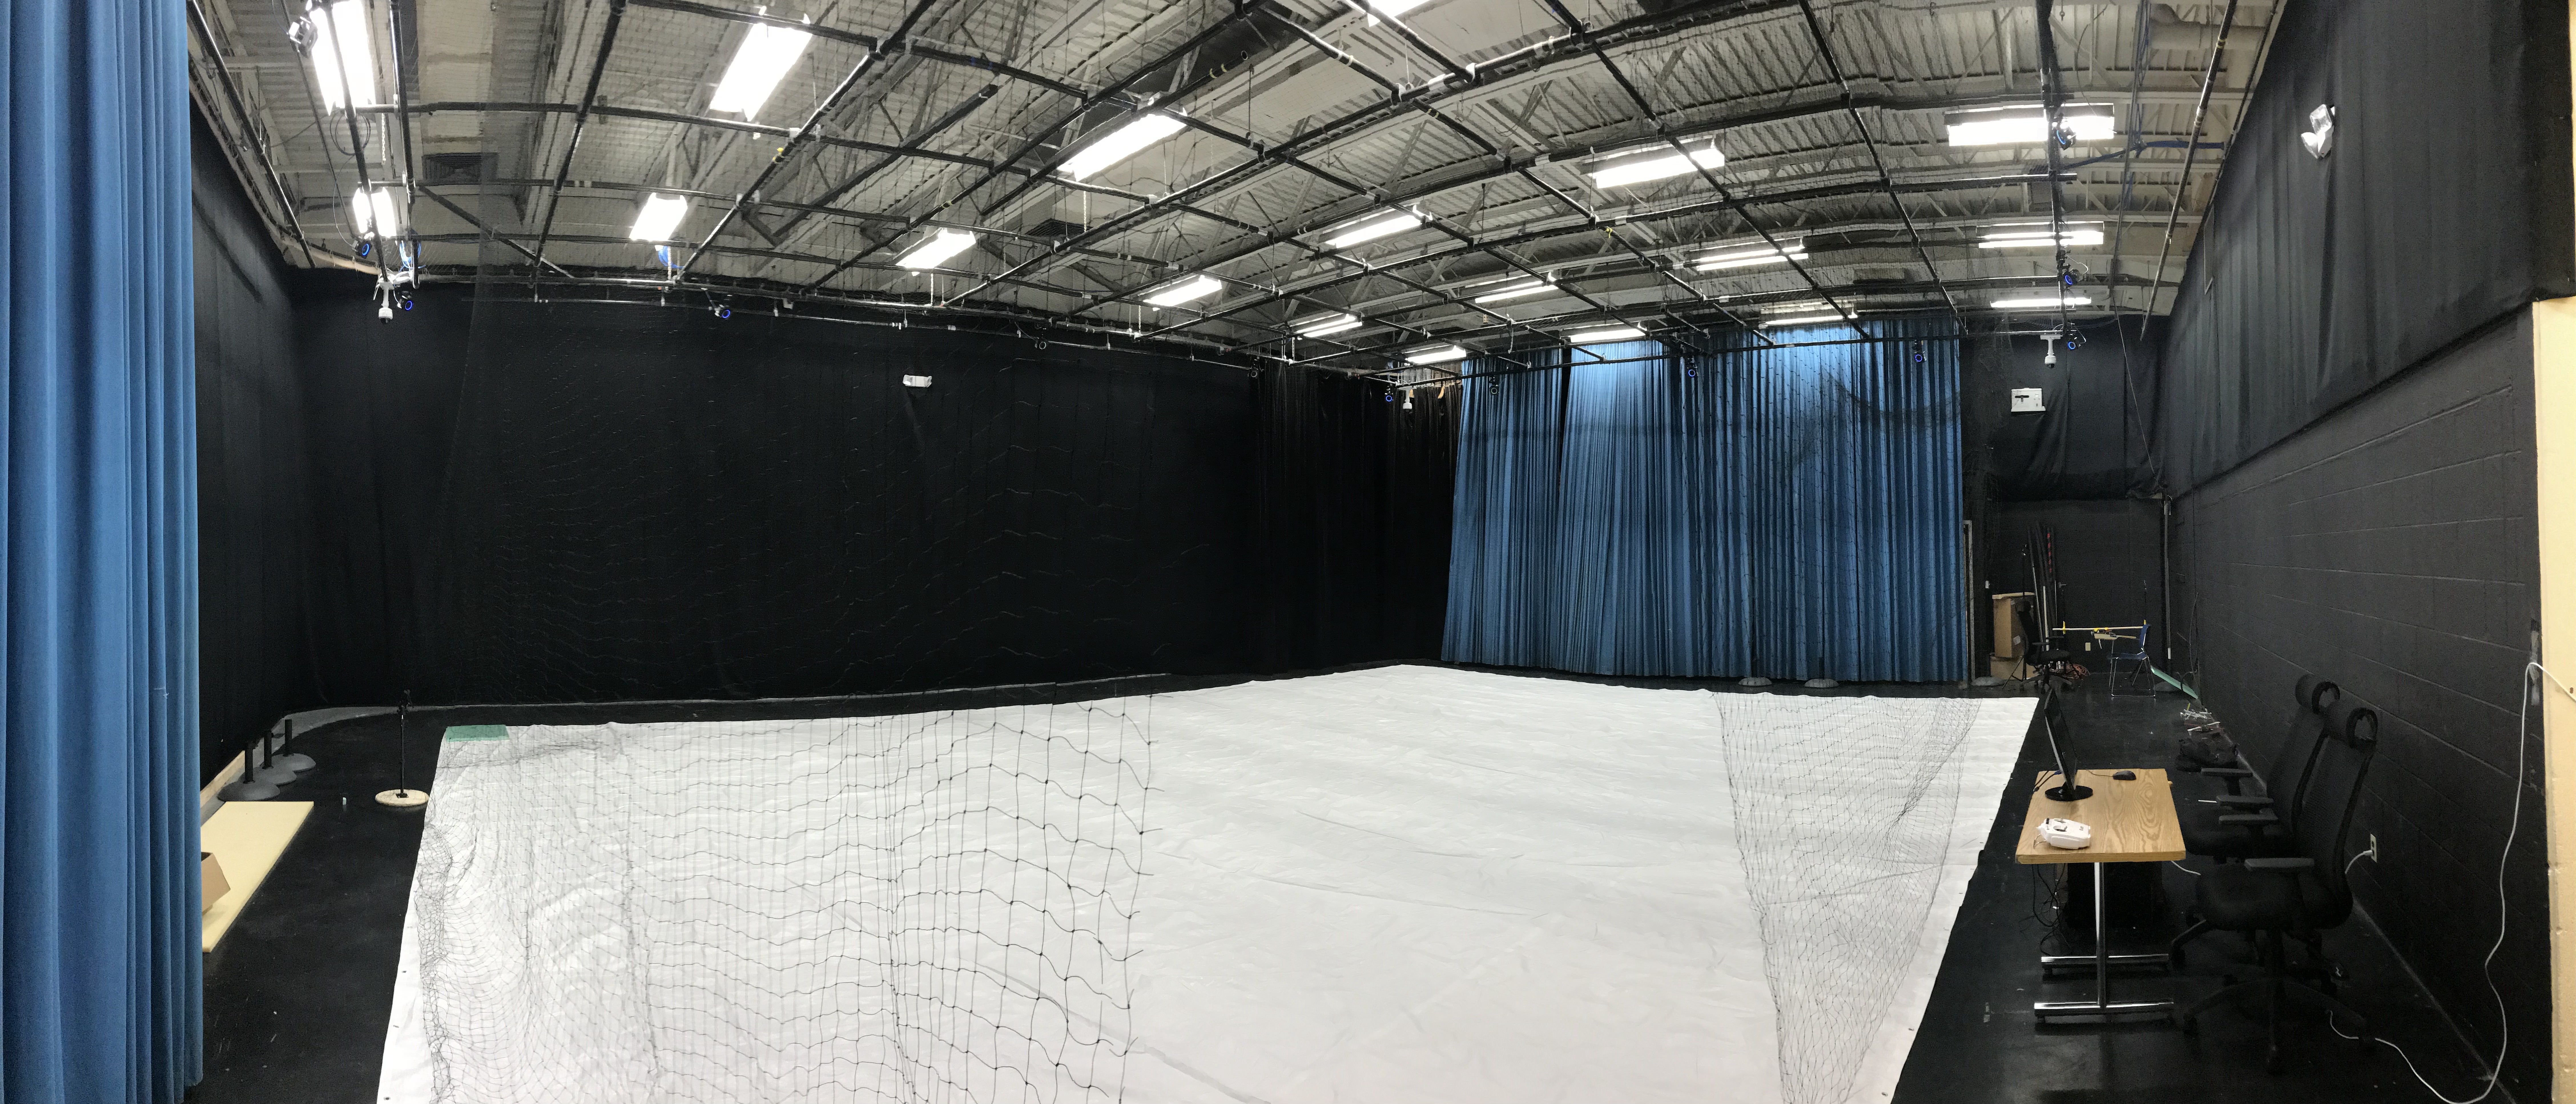
\includegraphics[width=1\textwidth]{IMG_1645} 
    \caption*{The LFMC Platform.}
\end{figure}
\begin{wrapfigure}{r}{0.35\textwidth} \vspace{-0.1in}
\center
    \includegraphics[width=0.35\textwidth]{IMAG1125} 
    \caption*{The Crazepony mini drone.}\vspace{-0.2in}
\end{wrapfigure}

\subsubsection*{The Artunis Project}
This is a model constructed and assembled at every level by the DCDS group. 
Artunis project, is constantly under development, and has not a particular frame yet. Its basic structure is as DJI F330 4-Axis RC Quadcopter Frame Kit, and it operates on ESP32 microcontrollers that are wifi enabled with a good amount of CPU power.  
 \begin{wrapfigure}{r}{0.35\textwidth}\vspace{-0.2in}
\center
    \includegraphics[width=0.35\textwidth]{IMAG1115} 
    \caption*{The Conference/Lab Room}\vspace{-0.2in}
\end{wrapfigure}
Artunis drones have undertaken the majority of the experimental missions designed and executed in the group, so far. 

The 1st Generation of Artunis encapsulates a ESP8266 wi-fi chip as the communication module. The embedded processor is 32bit STM32F427 Cortex M4 core with FPU, 168 MHz, and 256 KB RAM. Artunis's core is a small microcontroller with built-in wifi plus an Inertial Measurement Unit (IMU) sensor.

The 2nd Generation of Artunis is designed to use Hobbypower Pixhawk PX4 32Bit ARM Flight Controller with 8G SD Card for RC Multicopter FPV Quadcopter plus one Hobbypower strap.



\subsubsection*{The Aero Ready-to-Fly} This ready-to-fly unmanned aerial vehicle (UAV) development platform is a fully assembled, fully functional quadcopter powered by the Intel® Aero Compute Board. The Aero is equipped with Intel® RealSense™ depth and vision capabilities, running an open-source Linux operating system.  The advanced capabilities of Aero drones make them suitable for high precision experimental missions. For further information we refer to

 \texttt{https://click.intel.com/intel-aero-ready-to-fly-drone.html}.

\section*{Research Activities} Since its founding, the LFMC has been engaged in starting up a fully operating academic level test-bed. The first milestone was to establish compatible compartmental modules from all basic layers of experimental research. That is design, building and programming drones to efficiently communicate with the motion capture system and successfully execute experimental activities. % data-driven and control software library.   

\subsection*{State-Of-Art Research}
The current projects involve research along the following general directions: \begin{wrapfigure}{l}{0.35\textwidth}
\center
    \includegraphics[width=0.35\textwidth]{082317} 
    \caption*{The Artunis Drone.} \vspace{-0.9in}
\end{wrapfigure}
\begin{itemize}
\item Design feasible trajectories in $\mathbb R^3~\times ~SO(3)$ for drones.
\item Design a control for trajectory following.
\item Online Trajectory Generation.
\end{itemize} Preliminary experimental results and videos are published and available online on the departmental and the group's web-pages.
  
\subsection*{Future Research Associated with the Current Proposal}

The experimental division of DCDS group is currently engaged in developing the  3rd Generation of Artunis: \textit{A drone that can see and maneuver}. The next generation will be incorporate  the advanced properties:
 \begin{enumerate}
\item Fast Communication/Processing of Information
\item Exact Sensor Reading
\item Compact Design
\item Embedded Camera for Autonomous Vision-Based Control Laws.
\end{enumerate} 
 
The PI plans to develop a benchmark nonlinear network model for quadcopters platooning and implement a real-time risk analyzer in his drone lab. Our
ultimate goal is to develop real time data-driven risk analyzer that
can also be used in other disciplines such as robotics, transportation, energy, financial, and biological networks. This test-bed allows us for rigorous, transparent, and replicable testing and verification of the proposed unified theory of systemic risk measures for large-scale network of autonomous quadcopters.


The PI and his group members have been designing and assembling quadcopters from basic hardware elements. Currently, we are developing model-based maneuvering of individual quadcopter. Once we achieve this control objective, we will build a network of multiple quadcopters to form a platoon. With our current developments, we are anticipating to experience 2-4 mms of communication time delay. Also, when developing network models we will account for fluid field coupling among flying drones. In order to generate heavy-tailed disturbances, we will use an array of duck fans.
 
\begin{figure}[b]
\center
    \includegraphics[width=1\textwidth]{082318} \caption*{Experimentation and learning with the Artunis drones.}
\end{figure}


\subsection*{Staff Members}


The DCDS Lab is currently hosting more than 15 undergraduate, graduate, Ph.D. students and one postdoctoral scholar. 

\subsection*{Further Info}
For more information and updates on LFMC, visit the DCDS group web-page 

 \texttt{http://dcds.lehigh.edu/}, or contact Prof. Nader Motee.

\end{document}
